\documentclass[10pt]{article}
\usepackage{../../local}
\urlstyle{same}

\newcommand{\classcode}{Physics 110B}
\newcommand{\classname}{Electromagnetism and Optics II}
\renewcommand{\maketitle}{%
\hrule height4pt
\large{Eric Du \hfill \classcode}
\newline
\large{HW 05} \Large{\hfill \classname \hfill} \large{\today}
\hrule height4pt \vskip .7em
\small{Header styling inspired by Berkeley EECS Department: \url{https://eecs.berkeley.edu/}}
\normalsize
}
\linespread{1.2}
\begin{document}
	\maketitle
	\section*{Problem 1}
	\begin{enumerate}[label=(\alph*)]
		\item Show that the skin depth in a poor conductor (\( \sigma \ll \omega \epsilon) \)) is \( (2 /
			\sigma) \sqrt{\epsilon} / \mu \) (independent of the frequency). Find the skin depth (in meters)
			for (pure) water. (Use the static values of \( \epsilon, \mu \) and \( \sigma \); your answers
			will be valid only at relatively low frequencies.)

			\begin{solution}
				The skin depth is given by:
				\[
					d = \frac{1}{\kappa} = \frac{1}{\omega} \sqrt{\frac{2}{\epsilon \mu} }\left[ \sqrt{1 + \left(
					\frac{\sigma}{\epsilon \omega} \right)^2} - 1 \right]^{- 1 / 2}
				\]
				When \( \sigma \ll \omega \epsilon \), then we can make a Taylor approximation and use \( (1
				+ x)^{n} \approx 1 + n x \), so:
				\begin{align*}
					d &= \frac{1}{\omega}\sqrt{\frac{2}{\mu \epsilon}}\left[ 1 + \frac{1}{2}\left(
					\frac{\sigma}{\epsilon \omega} \right)^2 - 1 \right]^{- 1 / 2}\\
					&= \frac{1}{\omega}\sqrt{\frac{2}{\mu \epsilon}} \left[ \frac{1}{2}\left(
					\frac{\sigma}{\epsilon \omega} \right)^2 \right]^{- 1 / 2}\\
					&= \frac{1}{\omega}\sqrt{\frac{2}{\mu \epsilon}}\sqrt{2}\left( \frac{\epsilon
					\omega}{\sigma} \right) \\ 
					&= \frac{2}{\sigma}\sqrt{\frac{\epsilon}{\mu}} 
				\end{align*}
				as desired. For water, we have \( \epsilon = 80.2 \epsilon_0 \), \( \mu = 1.256 \times 10^{6}
				\) and \( \sigma = \frac{1}{8.3 \times 10^3} \). Plugging this in to Mathematica I get 8662 m.  
			\end{solution}
		\item Show that the skin depth in a good conductor (\( \sigma \gg \omega \epsilon \)) is \( \lambda /
			2\pi\) (where \( \lambda \) is the wavelength \textit{in the conductor}). Find the skin depth (in
			nanomoeters) for a typical metal (\( \sigma \approx 10^{7} (\mathrm{\Omega \cdot m})^{-1} \)) in
			the visible range (\( \omega \approx 10^{15} \text{/s} \)), assuming \( \epsilon \approx
			\epsilon_0 \) and \( \mu \approx \mu_0 \). Why are metals opaque?

			\begin{solution}
				First, we solve for \( d \) in a good conductor. Here, since \( \sigma \gg \omega \epsilon
				\), then the \( \frac{\sigma}{\omega \epsilon} \) term dominates so we have:
				\[
					d = \frac{1}{\omega}\sqrt{\frac{2}{\mu \epsilon}}\left( \frac{\epsilon \omega}{\sigma}
					\right) 
				\]
				Now, \( \lambda = \frac{2\pi}{k} \), and \( k \) is defined as:
				\[
					k = \omega \sqrt{\frac{\epsilon \mu}{2}} \left[ \sqrt{1 + \left( \frac{\sigma}{\epsilon
					\omega} \right)^2} + 1 \right]^{1 / 2}
				\]
				This is very similar to \( \kappa \), and under the approximation of a good conductor they
				become equal (the \( \pm 1 \) outside the square root becomes negligible). 
				Therefore, the wavelength is:  
				\[
					\lambda = \frac{2\pi}{\omega}\sqrt{\frac{2}{\mu \epsilon}} \left( \frac{\epsilon
					\omega}{\sigma} \right) = 2\pi d
				\]
				Thus, we get \( d = \frac{\lambda}{2\pi} \), as desired. For a metal, I get \( 3.362 \times
				10^{-9} \) m. This shows why metals are opaque, as the skin depth is on the order of
				nanometers.  
			\end{solution}
		\item Show that in a good conductor the magnetic field lags the electric field by \( 45^{\circ} \),
			and find the ratio of their amplitudes. For a numerical example, use the "typical metal" in part
			(b).  

			\begin{solution}
				In a good conductor, as we've seen in the previous example, we have \( k \approx \kappa \),
				and since \( \phi = \tan^{-1}\left( \frac{\kappa}{k} \right) \), then we have \( \phi \approx
				\tan^{-1}(1) = 45^{\circ} \). The ratio of the amplitudes is given by equation 9.139, which
				gives:
				\[
					\frac{B_0}{E_0} = \frac{K}{\omega} = \sqrt{\epsilon \mu \sqrt{1 + \left(
					\frac{\sigma}{\epsilon \omega} \right)^2}}
				\]
				Using the approximation of a good conductor, this simplifies to:
				\[
					\frac{K}{\omega} = \sqrt{\epsilon \mu \frac{\sigma}{\epsilon \omega}} =
					\sqrt{\frac{\sigma \mu}{\omega}}
				\]
				Plugging in the values for the "typical metal", we get \( 1.12 \times 10^{-7} \).
			\end{solution}
	\end{enumerate}

	\pagebreak
	\section*{Problem 2}
	\begin{enumerate}[label=(\alph*)]
		\item Calculate the (time-averaged) energy density of an electromagnetic plane wave in a conducting
			medium (Eq. 9.140). Show that the magnetic contribution always dominates. [\textit{Answer:} \(
			(k^2 / 2 \mu \omega^2) E_0^2 e^{-2 \kappa z} \).]

			\begin{solution}
				The total energy is given by:
				\[
					\int_{\mathcal{V}} \frac{1}{2}\epsilon_0|\mathbf{E}|^2 + \frac{1}{2\mu_0}|\mathbf{B}|^2
					\diff \tau 
				\]
				so the energy density is just the integrand. The real part of the waves (by Equation 9.138)
				is given by
				\begin{align*}
					\mathbf{E}(z, t) &= E_0e^{-\kappa z}\cos(kz - \omega t + \delta_E) \mathbf{\hat{x}}\\
					\mathbf{B}(z, t) &= B_0e^{-\kappa z}\cos(kz - \omega t + \delta_E + \phi) \mathbf{\hat{y}} 
					= \frac{K}{\omega}
					E_0e^{-\kappa z}\cos(kz - \omega t + \delta_E + \phi) \mathbf{\hat{y}}
				\end{align*}
				Therefore, the energy density is given by:
				\[
					U = \frac{1}{2}\left( \epsilon E_0^2 e^{-2\kappa z}\cos^2(kz - \omega t + \delta_E) +
					\frac{K^2}{\omega^2} E_0^2 e^{-\kappa z }\cos^2(kz - \omega t + \delta_E + \phi) \right)
				\]
				Averaged over time, the \( \cos^2(x) \) terms average out to \( \frac{1}{2} \), so we have
				\[
					U = \frac{1}{2}\left( \epsilon E_0^2 e^{-2\kappa z} \cdot \frac{1}{2} +
					\frac{1}{\mu}\frac{K^2}{\omega^2} E_0^2 e^{-2\kappa z} \cdot \frac{1}{2} \right)\\
				\]
				Factoring out terms and also replacing \( K^2 \) in terms of \( \mu, \omega \) and other
				terms:
				\begin{equation}
					\label{2:U}
					U = \frac{1}{4}E_0^2 e^{-2\kappa z}\left( \epsilon +
					\frac{1}{\mu}\frac{1}{\omega^2}\omega^2 \epsilon \mu\sqrt{1 + \left(
				\frac{\sigma}{\epsilon \omega} \right)^2} \right) = \frac{1}{4}E_0^2 e^{-2\kappa z} \epsilon
				\left( 1 + \sqrt{1 + \left( \frac{\sigma}{\epsilon \omega} \right)^2} \right)
				\end{equation}
				Finally, we note that the term in parentheses can be rewritten as \( \frac{2k^2}{\omega^2 \mu
				\epsilon} \), so finally:
				\[
					U = \frac{k^2}{2 \omega^2 \mu} E_0^2 e^{-2\kappa z}
				\]
				exactly as hinted at by the answer. Clearly the magnetic contribution dominates -- looking at
				\ref{2:U}, we see that the contribution is captured by the term in parentheses:
				\[
					1 + \sqrt{1 + \left( \frac{\sigma}{\epsilon \omega} \right)^2}
				\]
				The second term represents the magnetic contribution, which is far greater than the electric
				contribution represented by the first term. 
			\end{solution}
		\item Show that the intensity is \( (k / 2 \mu \omega) E_0^2 e^{-2 \kappa z} \). 

			\begin{solution}
				The intensity is given as the average power per unit area, so we have \( I = \mean{\mathbf{S}
				\cdot \mathbf{\hat{z}}}\). The Poynting vector is given by:
				\[
					\mathbf{S} = \frac{1}{\mu}(\mathbf{E} \times \mathbf{B}) = \frac{1}{\mu}\left(E_0
					\frac{K}{\omega}E_0 e^{-2\kappa z}\cos(kz - \omega t + \delta_E) \cos(kz - \omega t +
					\delta_E + \phi) \mathbf{\hat{z}}\right) 
				\]
				So the intensity is:
				\[
					I = \frac{E_0^2}{\mu}\frac{K}{\omega} e^{-2\kappa z}\mean{\cos(kz - \omega t + \delta_E)
					\cos(kz - \omega t + \delta_E + \phi)}
				\]
				The time average is calculated as:
				\[
					\mean{f} = \frac{1}{T}\int_{0}^{T} f(t) \diff t
				\]
				so in our case:
				\[
					\frac{1}{2\pi}\int_{0}^{2\pi}\cos(kz - \omega t + \delta_E) \cos(kz - \omega t + \delta_E
					+ \phi) \diff t
				\]
				Plugging this into Wolfram, we get:
				\[
					\mean{\cos(kz - \omega t + \delta_E) \cos(kz - \omega t + \delta_E + \phi)} =
					\frac{\cos\phi}{2}
				\]
				Thus, we have:
				\[
					I = \frac{1}{2}\frac{E_0^2}{\mu}\frac{K}{\omega} e^{-2\kappa z }\cos \phi
				\]
				Finally, we use the fact that \( K \cos \phi = k \), so therefore:
				\[
					I = \frac{k}{2 \mu \omega} E_0^2 e^{-2\kappa z}
				\]
				as desired. 
			\end{solution}
	\end{enumerate}
	\pagebreak
	\section*{Problem 3}
	Calculate the reflection coefficient for light at an air-to-silver interface (\( \mu_1 = \mu_2 = \mu_0,
	\epsilon_1 = \epsilon_0, \sigma = 6 \times 10^{7} (\mathrm{\Omega \cdot m})^{-1} \)), at optical
	frequencies (\( \omega = 4 \times 10^{15}\text{/s} \)). 

	\begin{solution}
		This problem literally just comes down to plugging in numbers. From equation 9.149, we know that
		\[
			E_{0R} = \left( \frac{1 - \tilde \beta}{1 + \tilde \beta} \right)E_{0I}
		\]
		so the reflection coefficient is given by:
		\[
			R = \left| \frac{1 - \tilde \beta}{1 + \tilde \beta} \right|^2
		\]
		where \( \tilde \beta = \frac{\mu_1v_1}{\mu_2v_2}\tilde k_2 \). Because \( \mu_2 = \mu_1 = \mu_0 \)
		and \( \epsilon_1 = \epsilon_0 \), then we have:
		\[
			\tilde \beta = \frac{1}{\sqrt{\mu_1 \epsilon_1} \omega} \tilde k_2
		\]
		We have \( \tilde k = k + i \kappa \), with \( k \) and \( \kappa \) as they are in equation 9.128,
		so from here it's just an exercise of plugging in numbers. I did this in Wolfram, which gave me a
		reflection of 0.933. Here's the code I used, since I feel like I really haven't shown enough work for
		this problem:
		\begin{center}
			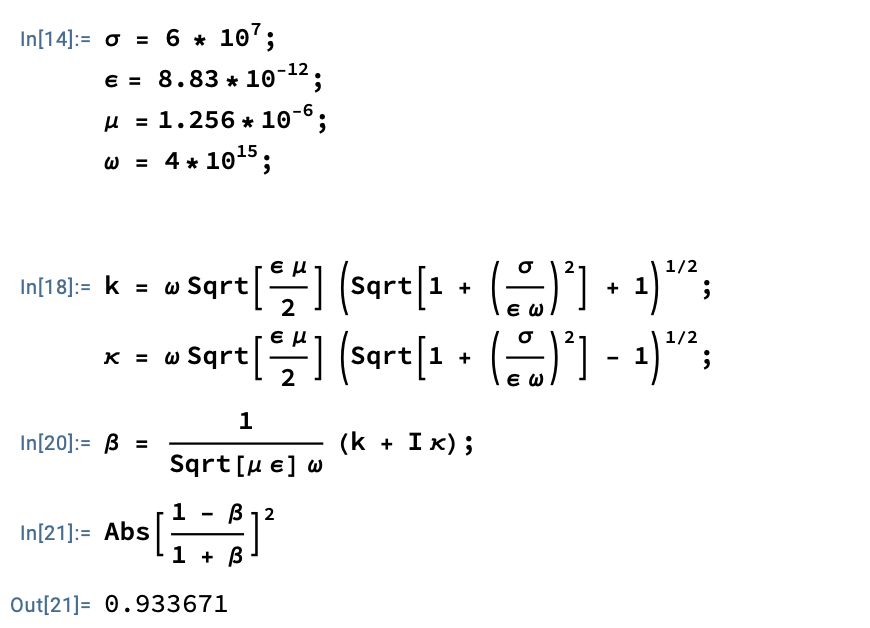
\includegraphics[scale=0.8]{q3.png}
		\end{center}
	\end{solution}
\end{document}
